\documentclass[tikz,border=10pt]{standalone}
\usepackage[utf8]{inputenc}
\usepackage{tikz}
\usepackage{xcolor}
\usetikzlibrary{positioning,backgrounds,fit}

% Define colors with cleaner palette matching the reference image
\definecolor{userLayerColor}{RGB}{153, 221, 204} % Light teal for User layer
\definecolor{apiLayerColor}{RGB}{255, 204, 179} % Light salmon for API layer
\definecolor{coreLayerColor}{RGB}{221, 238, 204} % Light green for Core layer
\definecolor{sequenceOpColor}{RGB}{242, 222, 242} % Light purple for Sequence Operations
\definecolor{imageOpColor}{RGB}{242, 222, 242} % Same light purple for Image Operations
\definecolor{fileFormatColor}{RGB}{222, 235, 247} % Light blue for File Format modules
\definecolor{utilityColor}{RGB}{238, 245, 219} % Very light green for Utility modules
\definecolor{arrowColor}{RGB}{100, 100, 100} % Dark gray for arrows

\begin{document}

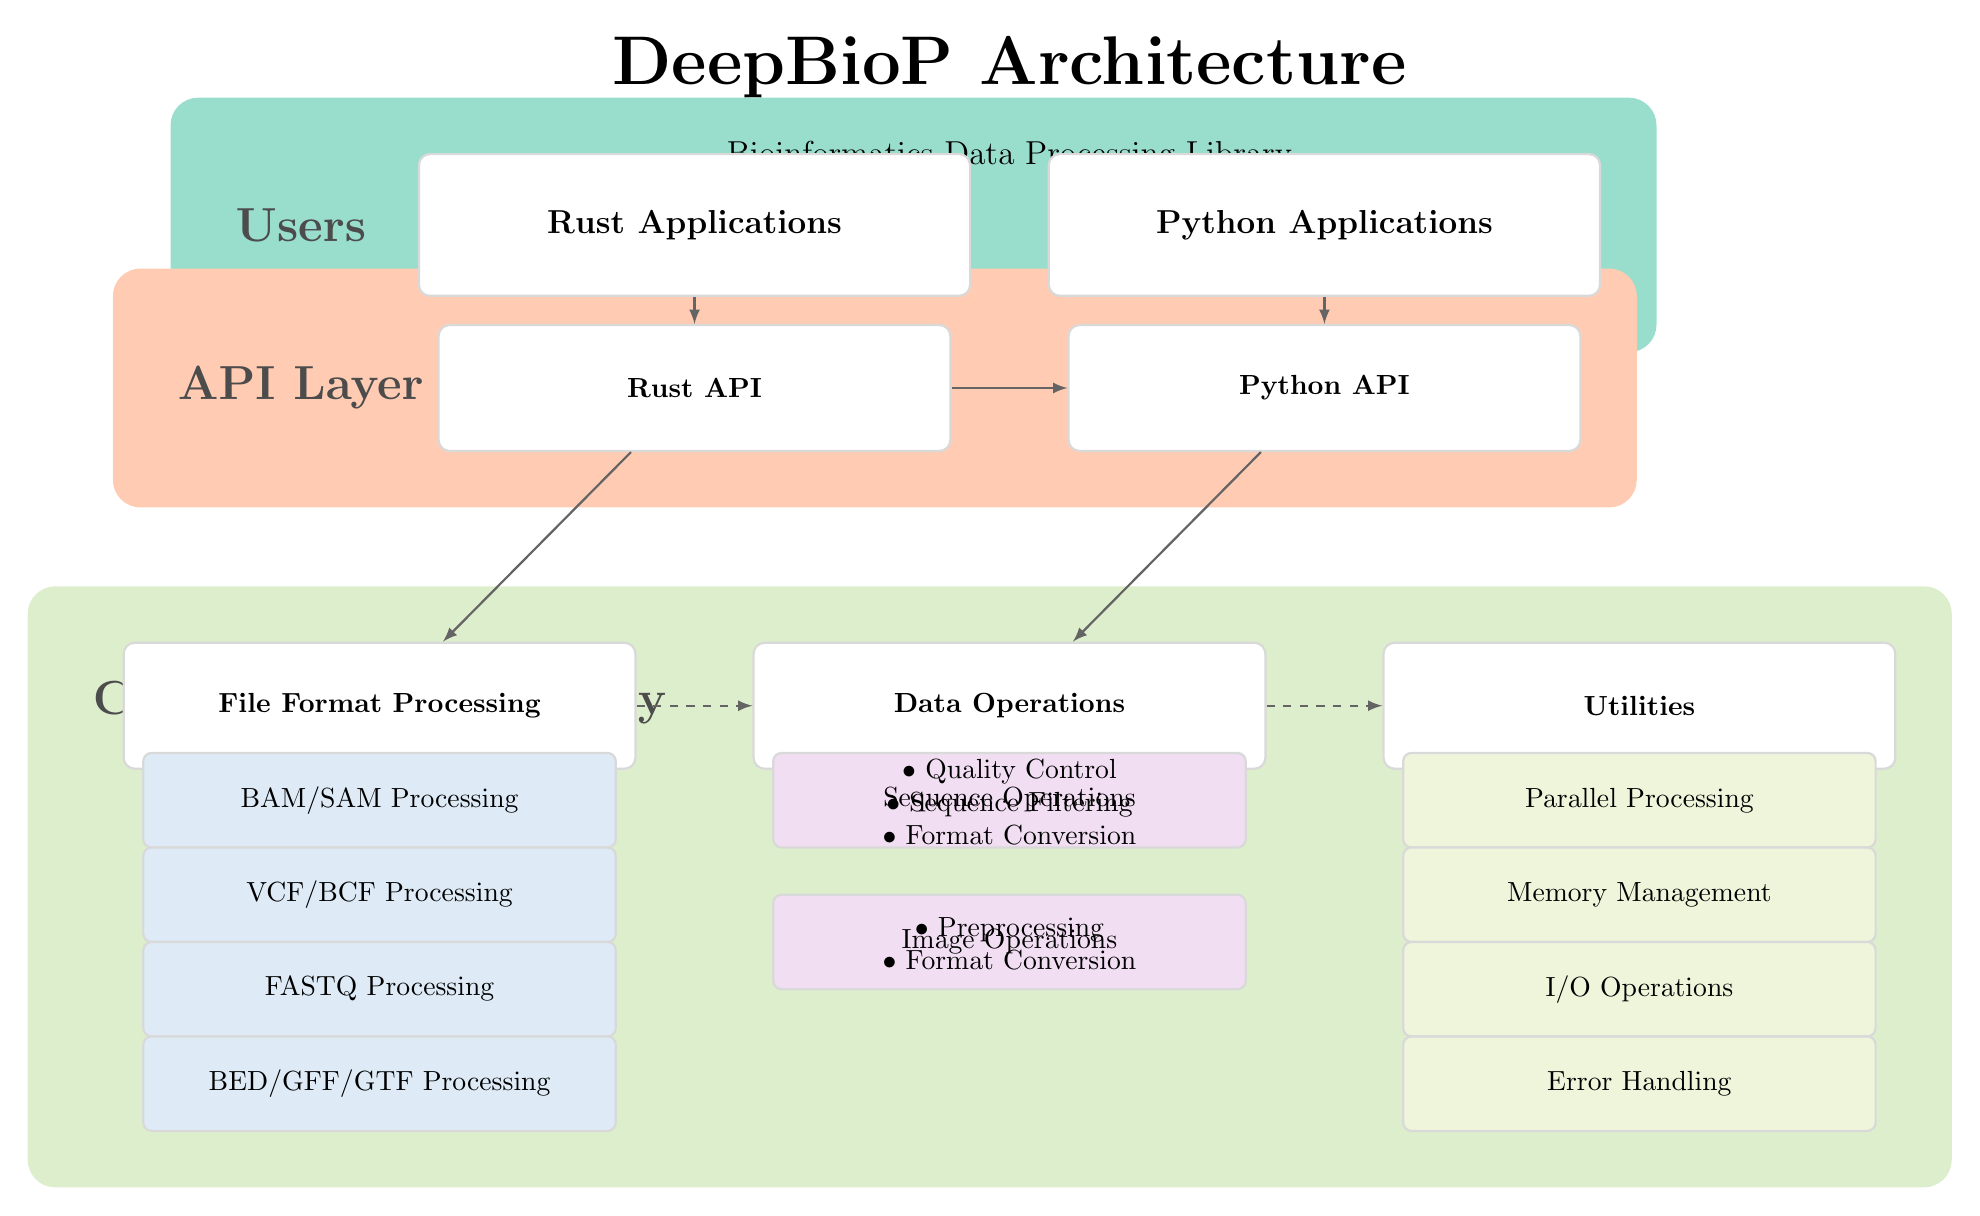
\begin{tikzpicture}[
		% Define styles for nodes
		mainmodule/.style={
				draw=gray!30,
				rectangle,
				minimum width=7cm,
				minimum height=1.8cm,
				rounded corners=4pt,
				thick,
				fill=white,
				font=\large\bfseries
			},
		submodule/.style={
				draw=gray!30,
				rectangle,
				minimum width=6.5cm,
				minimum height=1.6cm,
				rounded corners=4pt,
				thick,
				fill=white,
				font=\normalsize\bfseries
			},
		subsubmodule/.style={
				draw=gray!30,
				rectangle,
				minimum width=6cm,
				minimum height=1.2cm,
				rounded corners=3pt,
				thick,
				fill=#1
			},
		arrow/.style={
				->,
				thick,
				>=latex,
				draw=arrowColor
			},
		dashedarrow/.style={
				->,
				thick,
				>=latex,
				draw=arrowColor,
				dashed
			},
		layerlabel/.style={
				font=\LARGE\bfseries,
				text=black!70
			},
		layerbg/.style={
				fill=#1,
				rounded corners=10pt,
				inner sep=20pt
			}
	]

	% Title
	\node[font=\Huge\bfseries] (title) at (0,0) {DeepBioP Architecture};
	\node[font=\large, below=0.3cm of title] (subtitle) {Bioinformatics Data Processing Library};

	% Set up fixed vertical spacing
	\def\layerspacing{4cm}
	\def\modulespacing{1.2cm}

	% LAYER 1: Users Layer
	\node[layerlabel] (userlabel) at (-9,-2) {Users};

	% User layer modules
	\node[mainmodule] (rustapps) at (-4,-2) {Rust Applications};
	\node[mainmodule] (pythonapps) at (4,-2) {Python Applications};

	% LAYER 2: API Layer
	\node[layerlabel] (apilabel) at (-9, -2-\layerspacing) {API Layer};

	% API Layer modules
	\node[submodule] (rustapi) at (-4, -2-\layerspacing) {Rust API};
	\node[submodule] (pythonapi) at (4, -2-\layerspacing) {Python API};

	% LAYER 3: Core Processing Library
	\node[layerlabel] (corelabel) at (-8, -2-2*\layerspacing) {Core Processing Library};

	% Core layer - File Format Processing
	\node[submodule] (fileformat) at (-8, -2-2*\layerspacing-1) {File Format Processing};
	\node[subsubmodule=fileFormatColor] (bamsam) at (-8, -2-2*\layerspacing-1-\modulespacing*1) {BAM/SAM Processing};
	\node[subsubmodule=fileFormatColor] (vcfbcf) at (-8, -2-2*\layerspacing-1-\modulespacing*2) {VCF/BCF Processing};
	\node[subsubmodule=fileFormatColor] (fastq) at (-8, -2-2*\layerspacing-1-\modulespacing*3) {FASTQ Processing};
	\node[subsubmodule=fileFormatColor] (bedgffgtf) at (-8, -2-2*\layerspacing-1-\modulespacing*4) {BED/GFF/GTF Processing};

	% Core layer - Data Operations
	\node[submodule] (dataops) at (0, -2-2*\layerspacing-1) {Data Operations};
	\node[subsubmodule=sequenceOpColor] (seqops) at (0, -2-2*\layerspacing-1-\modulespacing*1) {Sequence Operations};

	% Add bullet points for Sequence Operations
	\node[text width=4.5cm, align=center] at (0, -2-2*\layerspacing-1-\modulespacing*1-0.6) {
		$\bullet$ Quality Control\\
		$\bullet$ Sequence Filtering\\
		$\bullet$ Format Conversion
	};

	\node[subsubmodule=imageOpColor] (imageops) at (0, -2-2*\layerspacing-1-\modulespacing*2.5) {Image Operations};

	% Add bullet points for Image Operations
	\node[text width=4.5cm, align=center] at (0, -2-2*\layerspacing-1-\modulespacing*2.5-0.5) {
		$\bullet$ Preprocessing\\
		$\bullet$ Format Conversion
	};

	% Core layer - Utilities
	\node[submodule] (utilities) at (8, -2-2*\layerspacing-1) {Utilities};
	\node[subsubmodule=utilityColor] (parallel) at (8, -2-2*\layerspacing-1-\modulespacing*1) {Parallel Processing};
	\node[subsubmodule=utilityColor] (memory) at (8, -2-2*\layerspacing-1-\modulespacing*2) {Memory Management};
	\node[subsubmodule=utilityColor] (io) at (8, -2-2*\layerspacing-1-\modulespacing*3) {I/O Operations};
	\node[subsubmodule=utilityColor] (error) at (8, -2-2*\layerspacing-1-\modulespacing*4) {Error Handling};

	% ARROWS: Connect the layers
	% User to API layer
	\draw[arrow] (rustapps) -- (rustapi);
	\draw[arrow] (pythonapps) -- (pythonapi);

	% API layer connection
	\draw[arrow] (rustapi) -- (pythonapi);

	% API to Core layer
	\draw[arrow] (rustapi) -- (fileformat);
	\draw[arrow] (pythonapi) -- (dataops);

	% Core layer internal connections
	\draw[dashedarrow] (fileformat) -- (dataops);
	\draw[dashedarrow] (dataops) -- (utilities);

	% BACKGROUND LAYERS
	\begin{pgfonlayer}{background}
		% Define fitting nodes for layer backgrounds with improved containment
		\node[fit=(rustapps)(pythonapps)(userlabel),
			layerbg=userLayerColor] (user-bg) {};

		\node[fit=(rustapi)(pythonapi)(apilabel),
			layerbg=apiLayerColor] (api-bg) {};

		\node[fit=(fileformat)(bedgffgtf)(dataops)(imageops)(utilities)(error)(corelabel),
			layerbg=coreLayerColor] (core-bg) {};
	\end{pgfonlayer}

\end{tikzpicture}

\end{document}
